\subsection{Rancangan \textit{Struktural}}
\label{subsec:arsitektur-struktural}

Arsitektur struktural yang digunakan ialah component \textit{diagram}. \textit{component} diagram menggambarkan dengan jelas hubungan antara sistem maupun subsistem yang ada. Sistem digambarkan dengan sebuah box dan module digambarkan dengan persegi panjang yang berada pada dalam box boxnya. Sistem utama dari \textit{remote deployment} hanya terdiri dari \textit{service} dan \textit{dashboard}. Sistem \textit{kubernetes cluster} sepenuhnya di atur oleh modul kubernetes yang ada pada sistem \textit{service}.

\begin{figure}[ht]
  \centering
  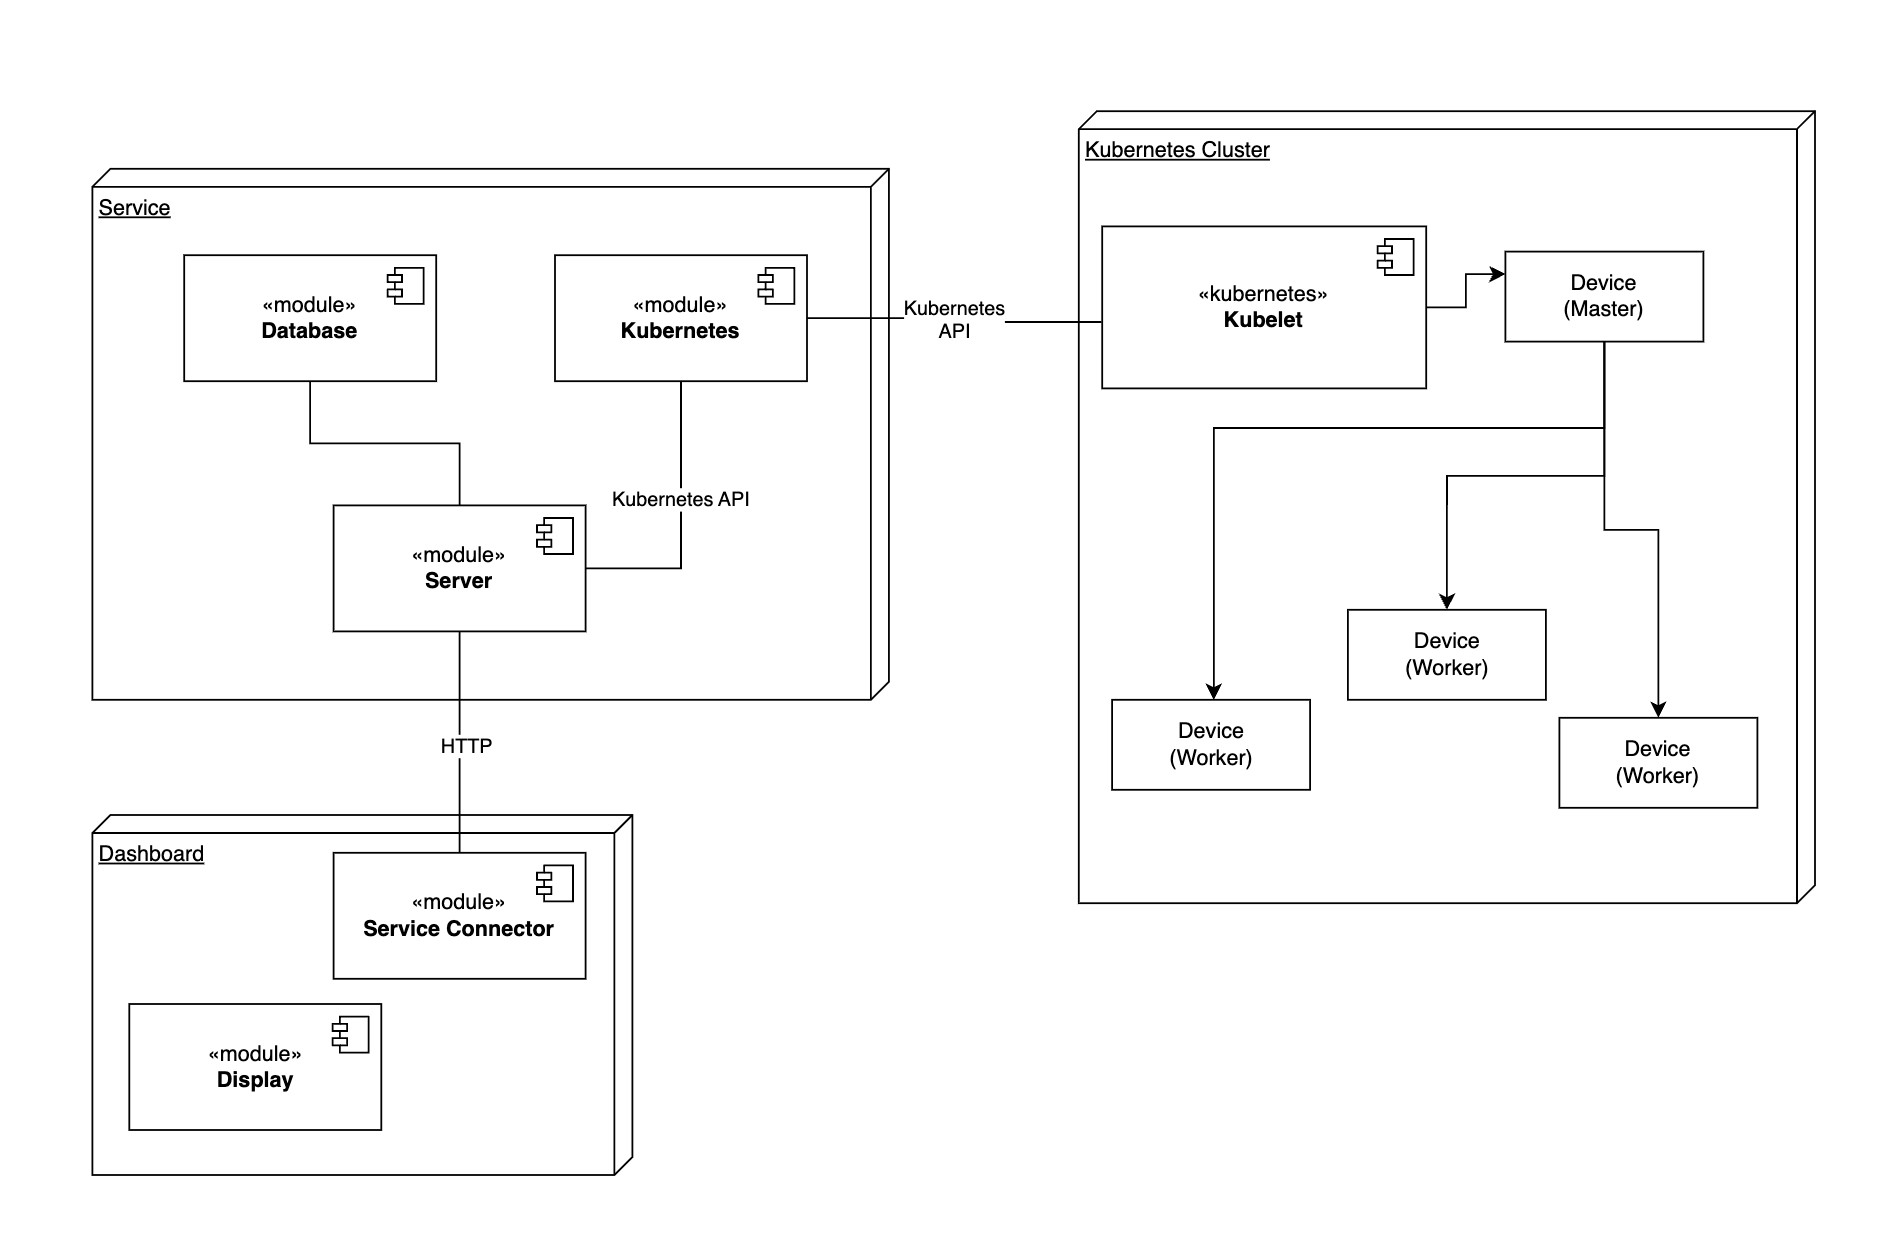
\includegraphics[width=1\textwidth]{resources/chapter-3/package-diagram.jpg}
  \caption{Package Diagram}
  \label{fig:package-diagram}
\end{figure}

